\subsection{Simulations}

\subsubsection{Effect of dataset dimensions}
\vspace{1.5cm}
\begin{table}[ht]
\centering
\begin{tabular}{l|l|rrrrrr}
\multicolumn{2}{l|}{} & \multicolumn{1}{c}{SpiecEasi} & \multicolumn{1}{c}{gCoda} & \multicolumn{1}{c}{ecoCopula} & \multicolumn{1}{c}{MRFcov} & \multicolumn{1}{c}{MInt} & \multicolumn{1}{c}{EMtree} \\ 
\hline
\multirow{3}{*}{{\rotatebox[origin=c]{90}{Easy}}} 
    & Cluster & 0.86  (0.20) & 0  (0.08) & 0.33  (0.14) & 0.74  (0.06) & 0.38  (0.17) & 0.12  (0.09) \\ 
    & Erdös   & 0.86  (0.21) & 0  (0.15) & 0.29  (0.15) & 0.73  (0.05) & 0.38  (0.15) & 0.12  (0.08) \\ 
    & Scale-free & 0.92  (0.04) & 0  (0.04) & 0.33  (0.11) & 0.88  (0.02) & 0.73  (0.09) & 0.34  (0.08) \\  \hline
\multirow{3}{*}{{\rotatebox[origin=c]{90}{Hard}}} & Cluster  &0.87  (0.12) & 0  (0.20) & 0.15  (0.18) & 0.78  (0.05) & 0.77  (0.09) & 0.36  (0.09) \\ 
 & Erdös.     & 0.88  (0.11) & 0  (0.24) & 0  (0.15) & 0.78  (0.05) & 0.77  (0.10) & 0.35  (0.09) \\ 
 & Scale-free & 0.94  (0.05) & 0  (0.13) & 0  (0.16) & 0.89  (0.03) & 0.94  (0.03) & 0.56  (0.07) \\ \hline
\end{tabular}
\caption{Medians and standard-deviation of FDR computed on 100 graphs of each type (\textit{easy}: $n=100, p=20$, \textit{hard}: $n=50, p=30$)}
\label{medFDR}
\end{table}

\begin{table}[ht]
\centering
\begin{tabular}{r|l|lllllll}
\multicolumn{2}{l|}{} & \multicolumn{1}{c}{SpiecEasi} & \multicolumn{1}{c}{gCoda} & \multicolumn{1}{c}{ecoCopula} & \multicolumn{1}{c}{MRFcov} & \multicolumn{1}{c}{MInt} & \multicolumn{1}{c}{EMtree} \\ \hline
\multirow{3}{*}{{\rotatebox[origin=c]{90}{Easy}}} &Cluster & 0.16  (0.11) & 0.05  (0.07) & 1.04  (0.48) & 2.26  (0.58) & 0.30  (0.13) & 0.62  (0.14) \\ 
& Erdös & 0.15  (0.09) & 0.06  (0.08) & 0.95  (0.50) &2.23  (0.42) & 0.30  (0.14) & 0.58  (0.12) \\ 
 & Scale-free & 0.63  (0.13) & 0.08  (0.07) & 0.92  (0.30) &4.86  (0.44) & 0.81  (0.25) & 0.96  (0.08) \\ \hline
\multirow{3}{*}{{\rotatebox[origin=c]{90}{Hard}}}  & Cluster & 0.21  (0.08) & 0.02  (0.03) & 0.02  (0.17) & 1.65  (0.33) & 0.68  (0.30) & 0.43  (0.10) \\ 
 & Erdös & 0.21  (0.08) & 0.02  (0.02) & 0.00  (0.18) & 1.56  (0.32)& 0.66  (0.25) & 0.42  (0.10) \\ 
 & Scale-free & 0.61  (0.12) & 0.04  (0.03) & 0.08  (0.24) &3.29  (0.40) & 3.63  (1.08) & 0.94  (0.09) \\ 
   \hline
\end{tabular}

\caption{Medians and standard-deviation of density ratio computed on 100 graphs of each type (\textit{easy}: $n=100, p=20$, \textit{hard}: $n=50, p=30$)}
\label{meddens}
\end{table}

\begin{table}[ht]
\centering
\begin{tabular}{l|l|rrrrrr}
\multicolumn{2}{l|}{} & \multicolumn{1}{c}{SpiecEasi} & \multicolumn{1}{c}{gCoda} & \multicolumn{1}{c}{ecoCopula} & \multicolumn{1}{c}{MRFcov} & \multicolumn{1}{c}{MInt} & \multicolumn{1}{c}{EMtree} \\ \hline
\multirow{3}{*}{{\rotatebox[origin=c]{90}{Easy}}} & Cluster & 1.77 & 13.89 & 1.74 & 0.00 & 0.00 & 0.00 \\
 & Erdös & 0.68 & 11.95 & 0.99 & 0.00 & 0.83 & 0.00 \\
 & Scale-free & 0.00 & 1.88 & 0.00 & 0.00 & 0.00 & 0.00 \\ \hline
\multirow{3}{*}{{\rotatebox[origin=c]{90}{Hard}}} & Cluster & 0.00 & 14.05 & 23.40 & 0.00 & 0.00 & 0.00 \\
 & Erdös & 0.00 & 20.85 & 27.28 & 0.00 & 0.00 & 0.00 \\
 & Scale-free & 0.00 & 5.97 & 15.46 & 0.00 & 0.00 & 0.00 \\ \hline
\end{tabular}
\caption{Percentage of empty networks computed on 100 graphs of each type (\textit{easy}: $n=100, p=20$, \textit{hard}: $n=50, p=30$)}
\label{empty}
\end{table}

\newpage

\begin{table}[ht]
\centering
\begin{tabular}{lrrrrrr}
 & \multicolumn{1}{c}{SpiecEasi} & \multicolumn{1}{c}{gCoda} & \multicolumn{1}{c}{ecoCopula} & \multicolumn{1}{c}{MRFcov} & \multicolumn{1}{c}{MInt} & \multicolumn{1}{c}{EMtree} \\ 
  \hline
Easy & 29.73  (2.00) & ~1.29  (~0.30) & 28.14  (1.46) & 48.7  (2.32) & 138.13  (39.60) & 50.19  (7.81) \\ 
  Hard & 29.38  (1.31) & 40.73  (20.94) & 27.16  (1.30) & 14.1  (0.36) & ~95.27  (46.34) & 23.59  (2.09) \\ 
   \hline
\end{tabular}
\caption{Median and standard-deviation of running times in seconds  for scale-free structures, for two dataset dimensions (\textit{easy}: $n=100$, $p=20$, \textit{hard}: $n=50$, $p=30$). }
\label{timeSF}
\end{table}

\vspace{1.5cm}

\begin{figure}[H]
    \centering
    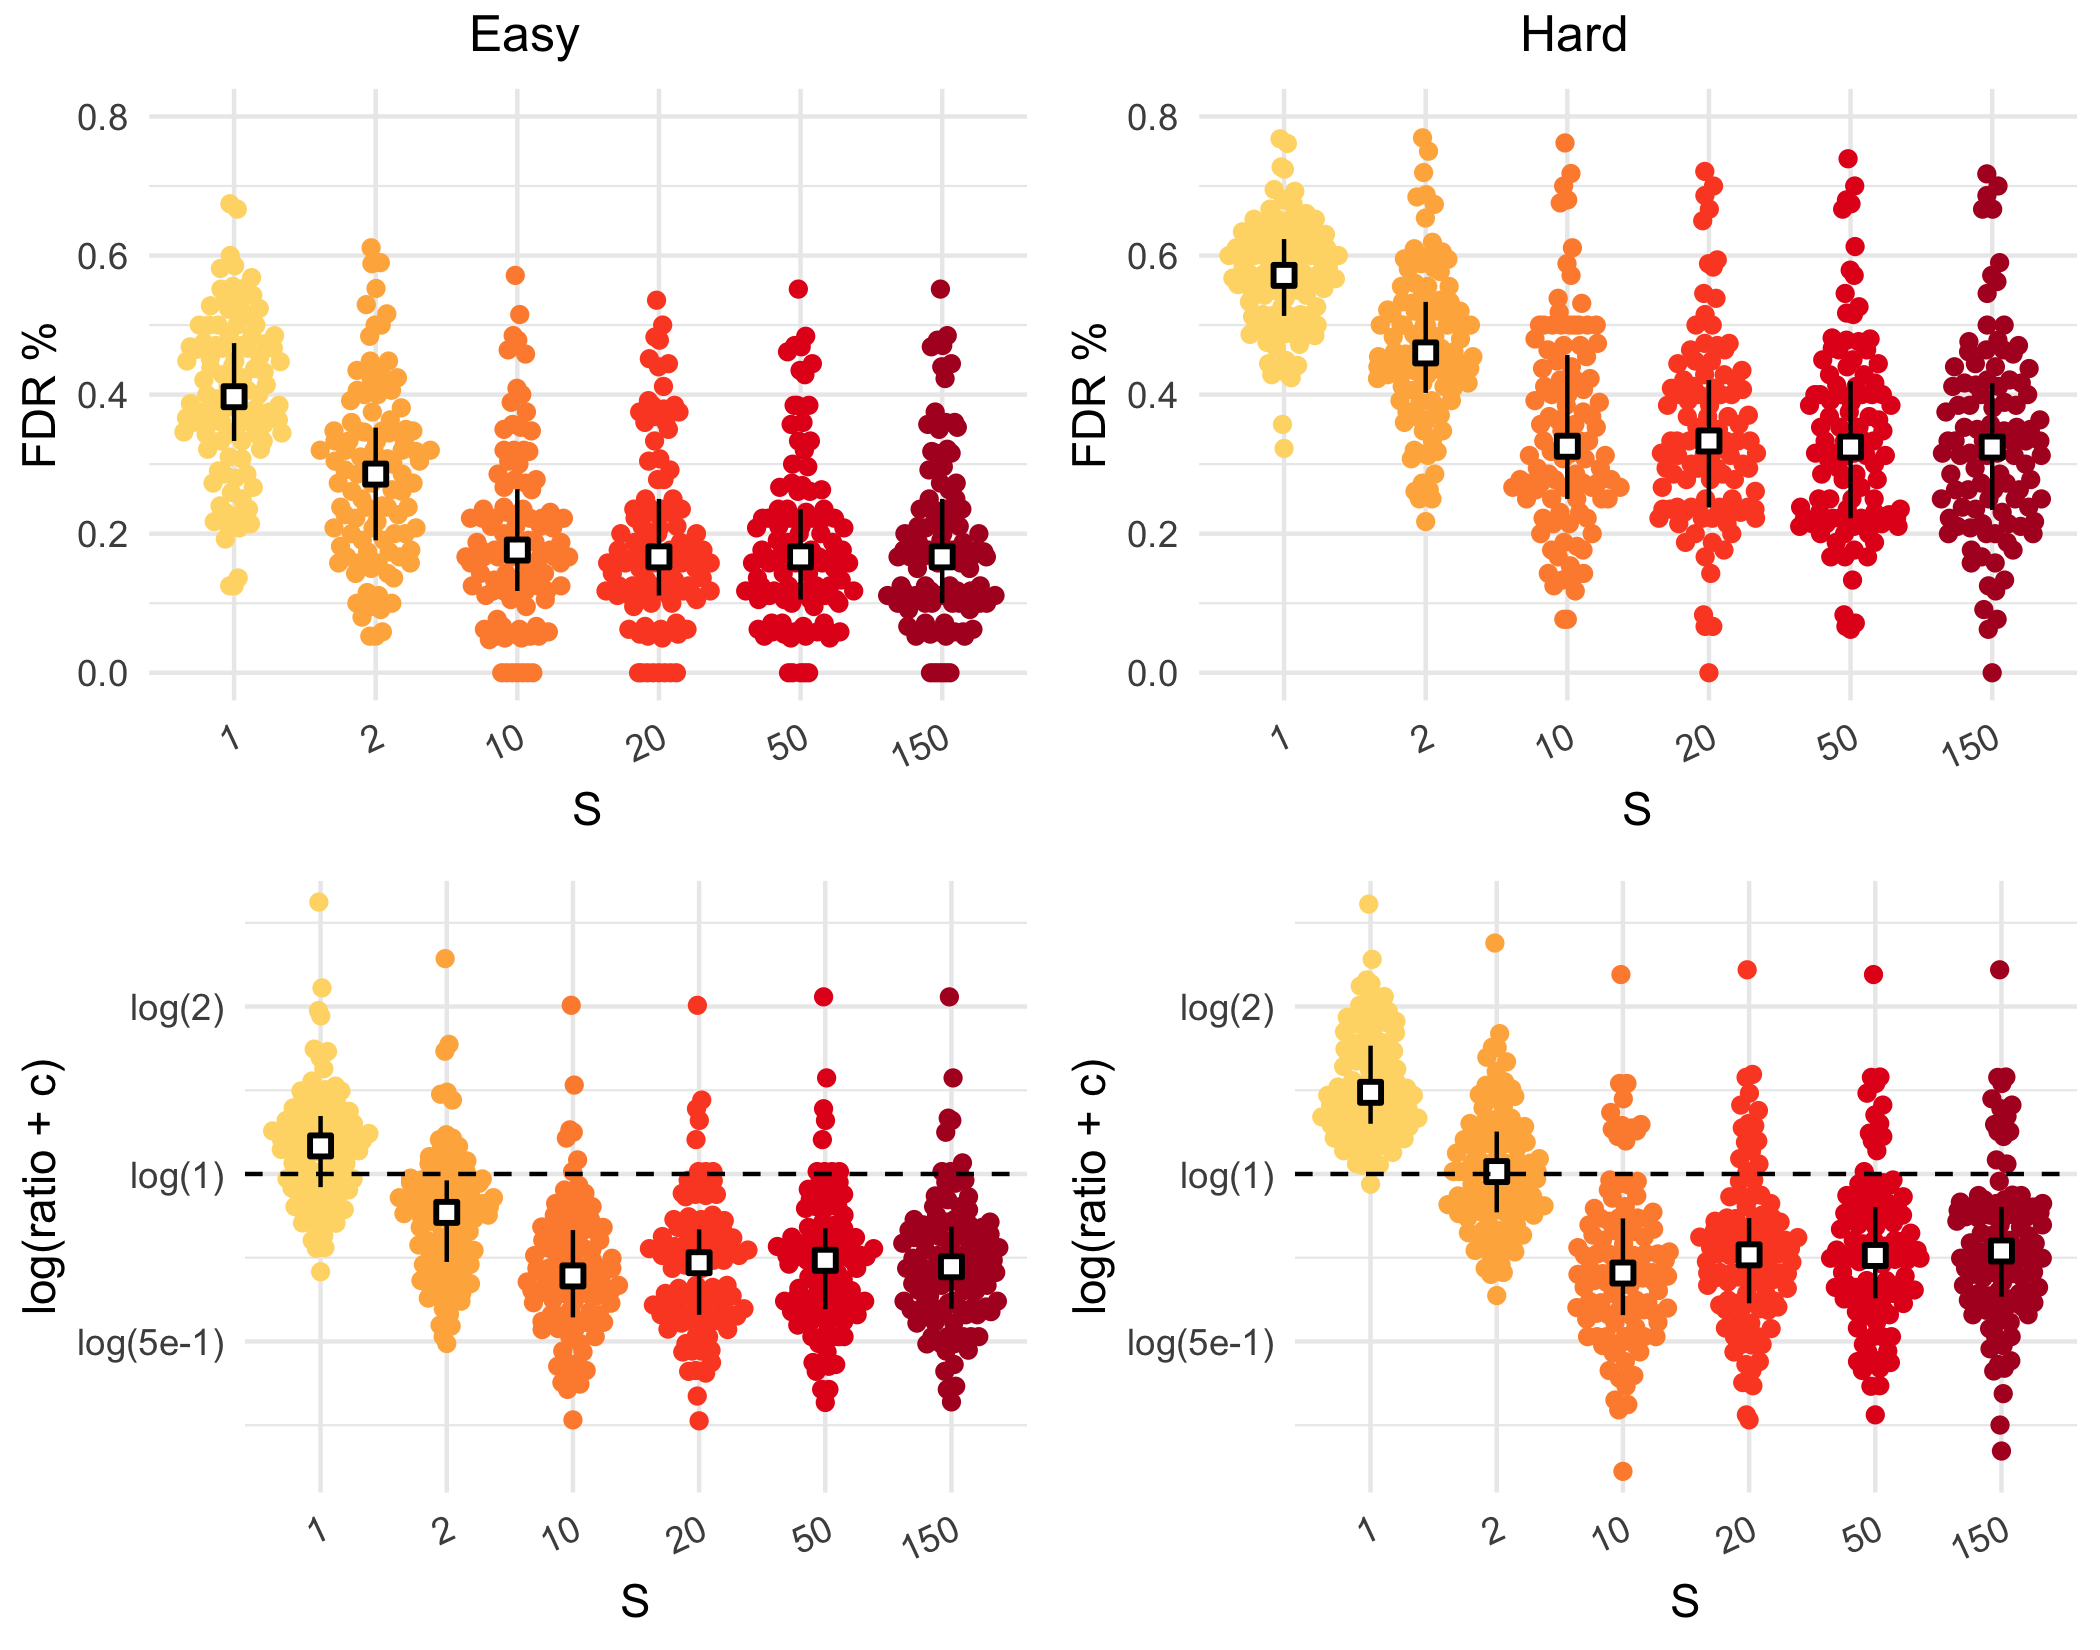
\includegraphics[width=10cm]{figs/S_effect.png}
    \caption{FDR and density ratio measures of EMtree with varying values of number of sub-samples $S$ (Erdös structure).}
    \label{Seffect}
\end{figure}


\begin{table}[ht]
\centering
\begin{tabular}{l|rrrrrr}
  $S$ & \multicolumn{1}{c}{1} & \multicolumn{1}{c}{2} & \multicolumn{1}{c}{10} & \multicolumn{1}{c}{20} & \multicolumn{1}{c}{50} & \multicolumn{1}{c}{150} \\ \hline
  Easy & 0.66  (0.15) & 1.86  (0.23) & 7.00  (0.81) & 12.29  (1.27) & 29.50  (3.39) & 87.30  (10.36) \\ 
  Hard & 0.45  (0.12) & 1.44  (0.14) & 5.06  (0.78) & 8.97  (0.87) & 23.35  (2.40) & 69.29  (10.83) \\ 
   \hline
\end{tabular}
\caption{Median and standard-deviation running-time values in seconds for inference of Erdös structure with EMtree and different values of the number of sub-samples $S$.}
\label{timesS}
\end{table}

\subsubsection{Effect of network density}

\begin{table}[H]
\centering
\begin{tabular}{l|rr|rr}
    & \multicolumn{1}{c}{$n < 50$} & \multicolumn{1}{c}{$n\geq 50$} & \multicolumn{1}{c}{$p < 20$} & \multicolumn{1}{c}{$p\geq 20$} \\  \hline
  EMtree    &   0.41 (0.11)	&   0.60 (0.15) &   0.38 (0.12) &    0.71 (0.21)      \\ 
  gCoda     &   0.12 (0.47)	&   0.07 (0.03) &   0.05 (0.03) &    0.09 (0.06)     \\ 
  SpiecEasi &   2.41 (0.25)	&   2.41 (0.25) &   2.39 (0.25) &    2.42 (0.25)      \\ 
   \hline
\end{tabular}
\caption{Median and standard-deviation of running times for each method in seconds, for $n$ and $p$ parameters. corresponding to Erdös and cluster structures with $5/p$ densities.}
\label{timeDenser}
\end{table}

\newpage
\subsection{Illustrations}
\subsubsection{Effect of the edge frequency threshold}

\begin{figure}[H]
    \centering
    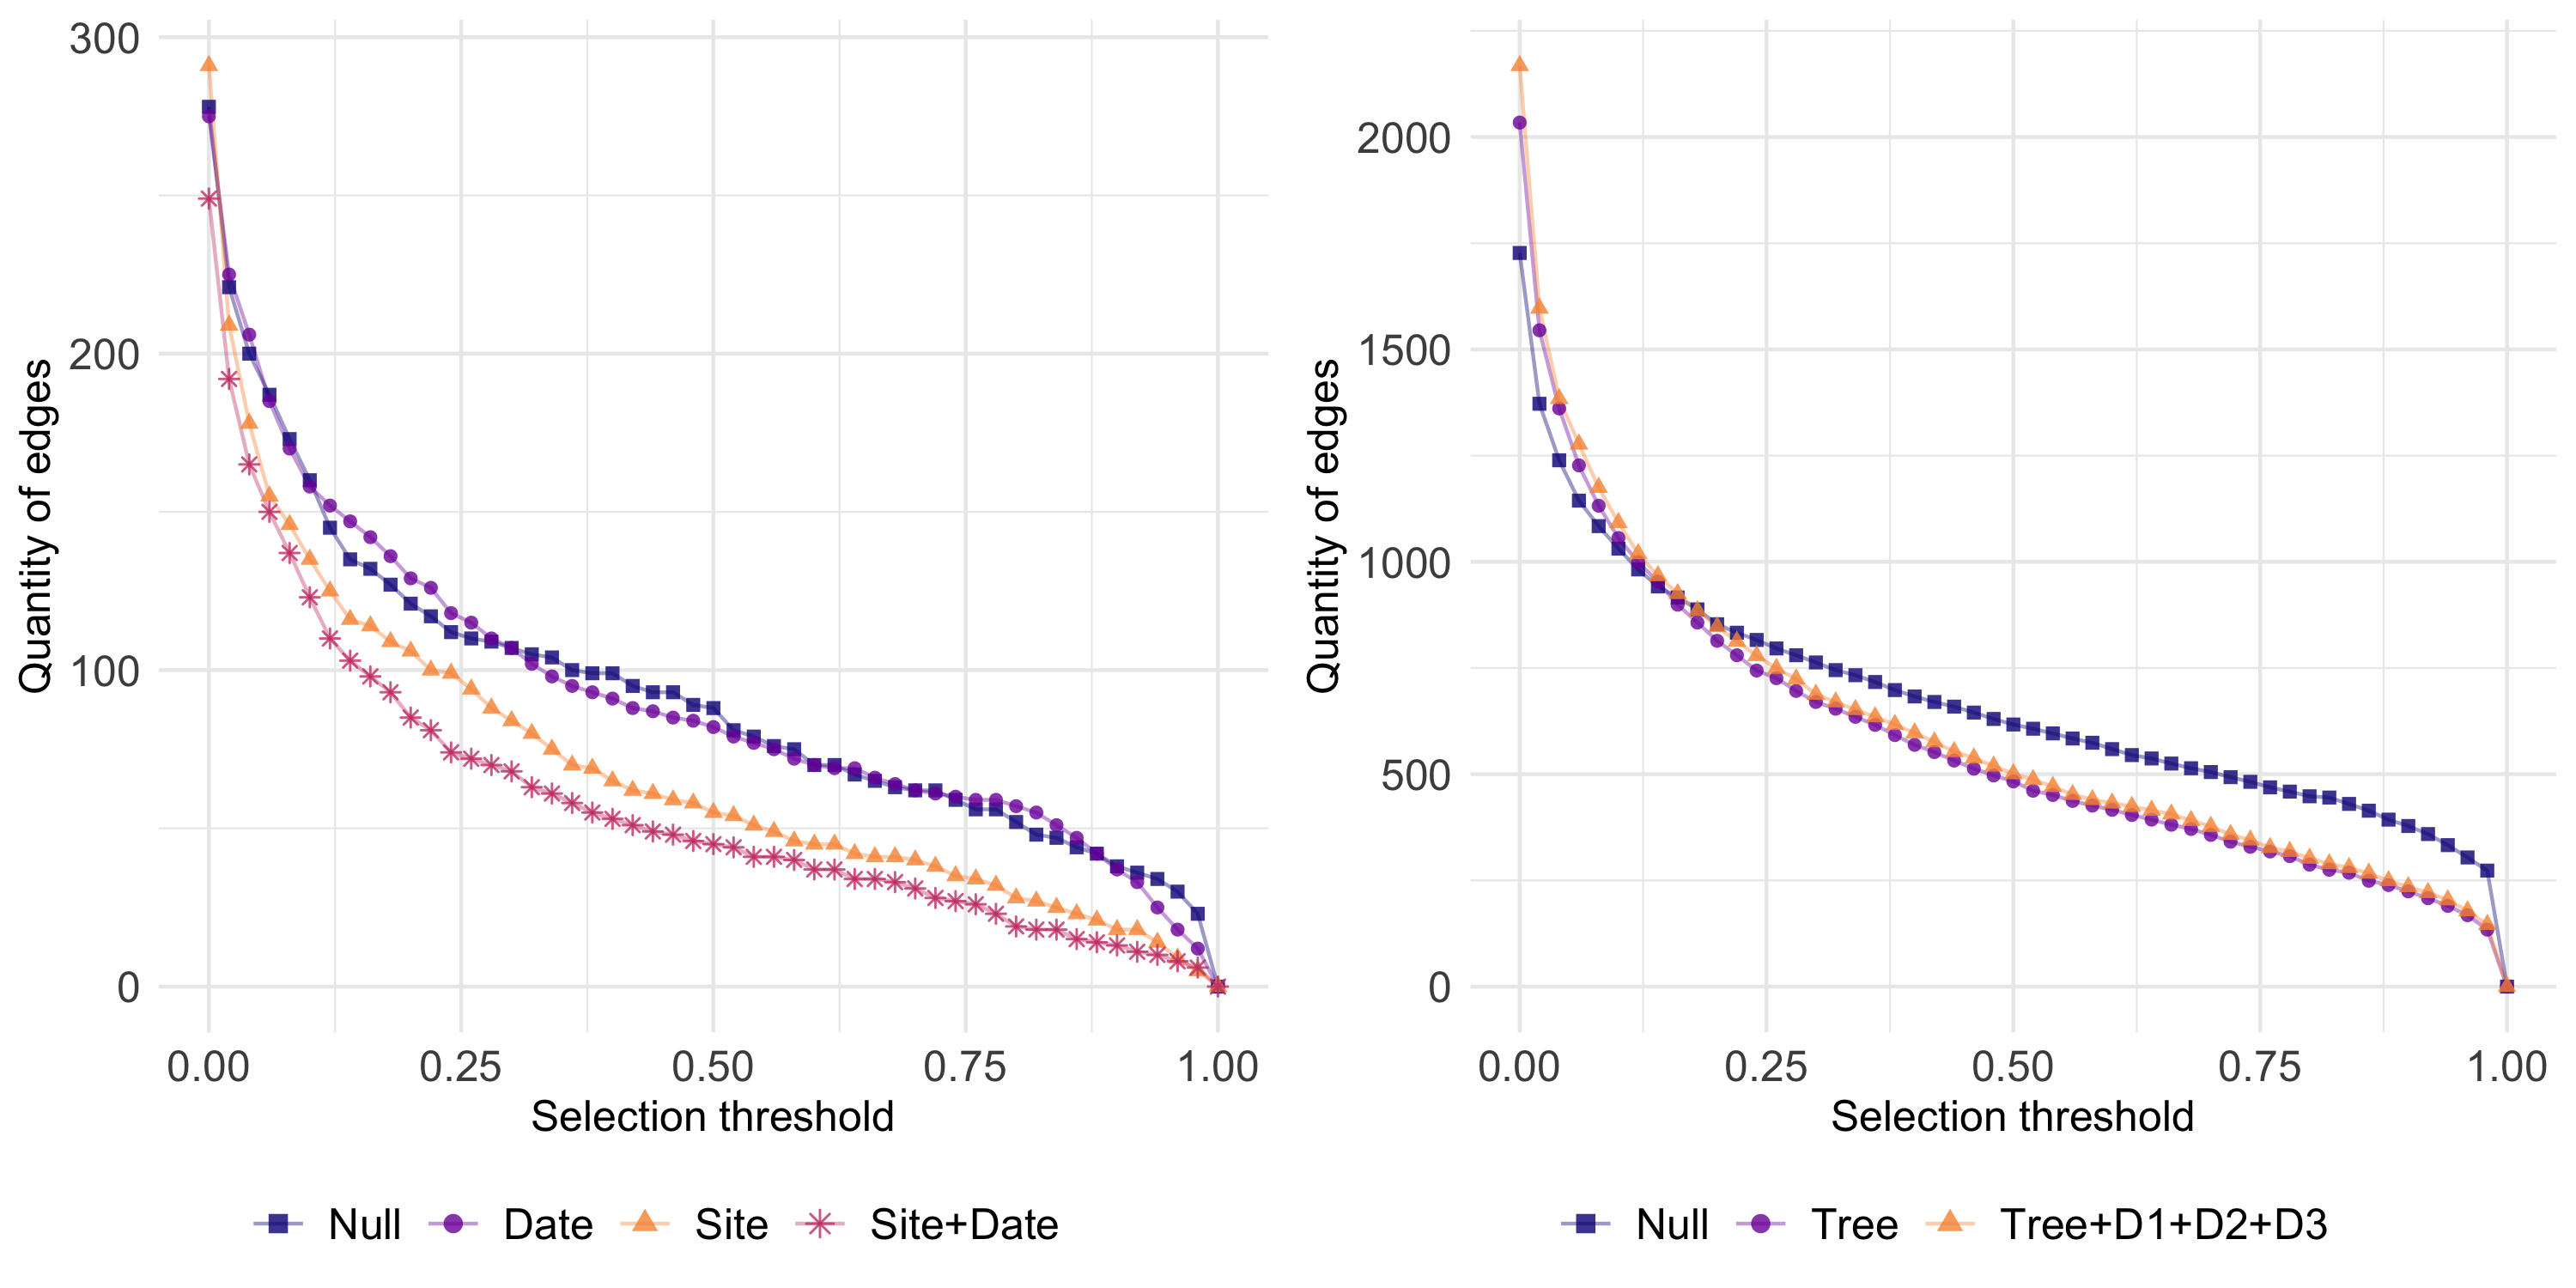
\includegraphics[width=\linewidth]{figs/QET_twoDataSets.png}
    \caption{Quantity of selected edges as a function of the selection threshold (\textit{left}: Fatala fishes, \textit{right}: oak mildew.)}
    \label{QETOak}
\end{figure}

The curves displayed on Fig. \ref{QETOak} are very smooth, which illustrates the difficulty of setting this threshold.


\subsubsection{Fatala River fishes}
\label{names_Baran}
\paragraph{Species names with highest betweenness scores:}
  13: Galeoides decadactylus; 19: Liza grandisquamis, 22:  Pseudotolithus brachygnatus, 25: Pellonula leonensis, 27:  Polydactylus quadrifilis, 30: Pseudotolithus typus, 32: Tylochromis intermedius.
